\documentclass[paper=a4paper,fontsize=10pt,jafontscale=0.925,twocolumn]{jlreq}
\usepackage{luatexja}
\usepackage{lab-handout}
\usepackage{graphicx} % Added for includegraphics

% ここから上は変更しない

\title{VRホラー体験時におけるマルチモーダル生体情報を用いた実時間感情推定} % 自身の卒業研究/修士論文の予定表題に変更

%以下は適切な所属を1つ選択
%\affiliation{人間システム工学科 井村研究室} % 卒業研究(人間システム工学科)
\affiliation{知能・機械工学課程 井村研究室} % 卒業研究(知能・機械工学課程)
%\affiliation{人間システム工学専攻 井村研究室} % 修士論文

\studentnumber{27020856} % 8桁の学籍番号
\author{趙 聖化} % 姓名間の空白は半角で

\graphicspath{{./}} % 画像を置いておくフォルダ名

\begin{document}

\maketitle

% ----- 図1(flowchart)のブロックを削除しました -----
% \begin{figure}[tp]
%  \centering
%  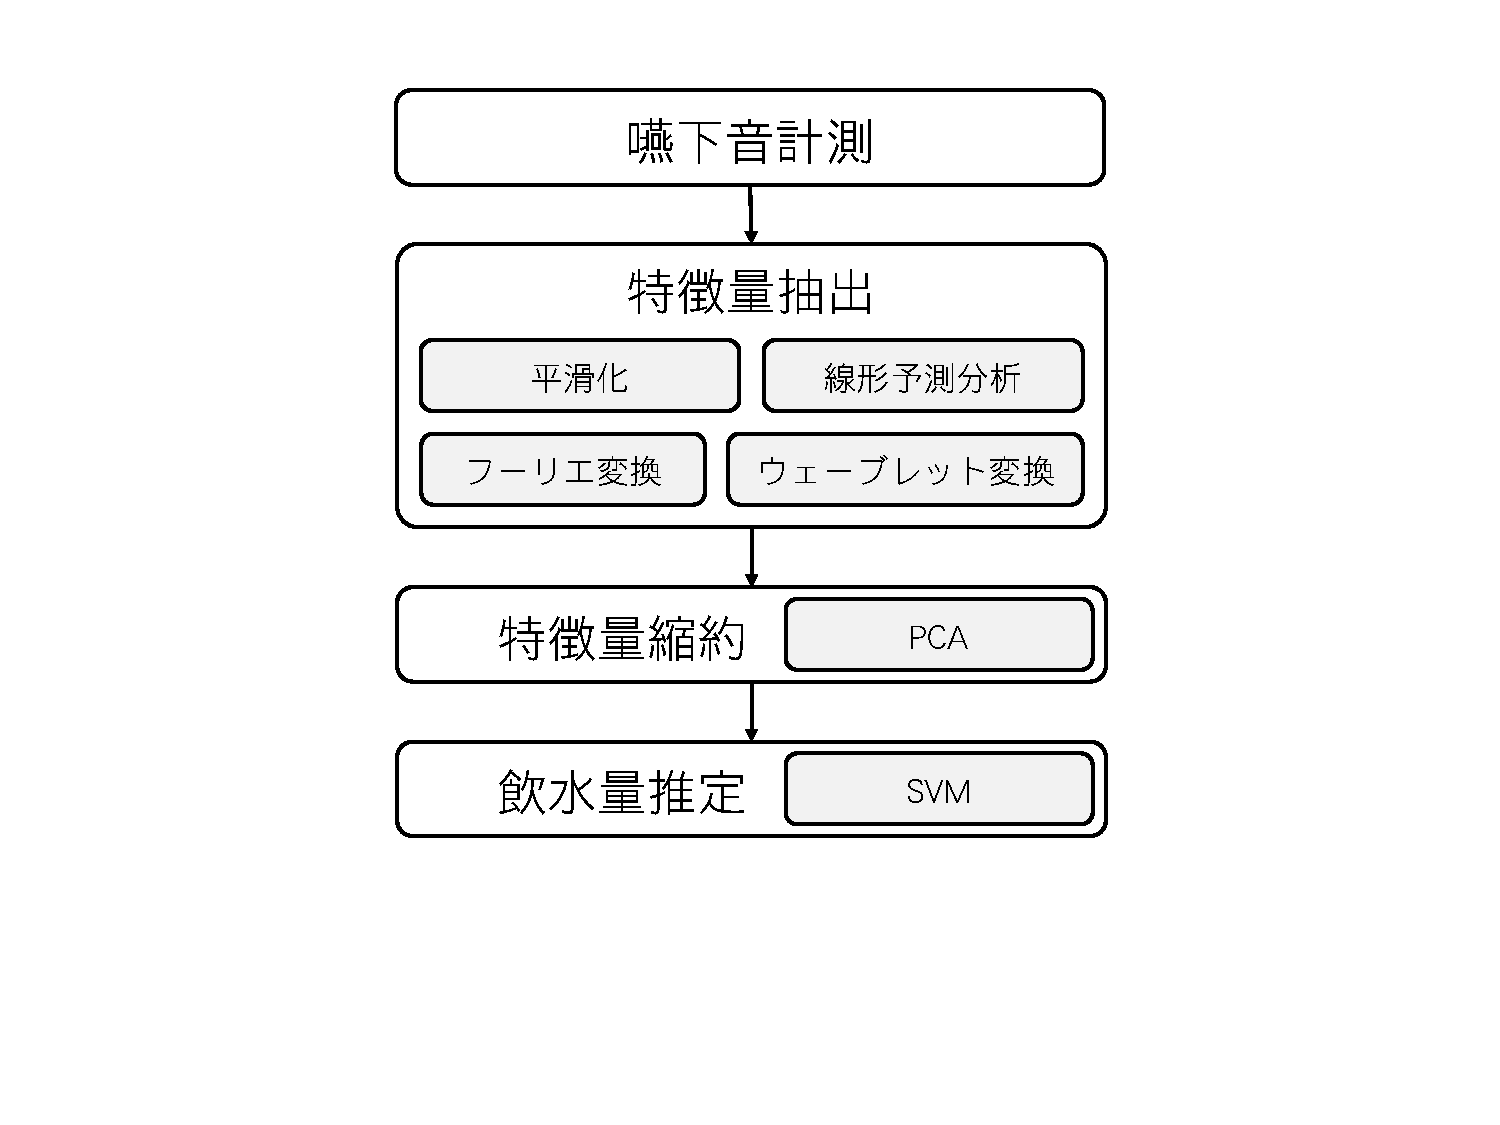
\includegraphics[width=\columnwidth]{flowchart.pdf}
%  \caption{提案する感情推定システムの処理フロー}
%  \label{fig:flow}
% \end{figure}

\section{はじめに}

VRは,その強い没入感からユーザの感情を効果的に喚起する媒体として,感情研究の分野で広く利用されている 。本研究では,VR体験の中でも特に強い情動反応を引き起こすホラーコンテンツに着目する。視線追跡機能付きHMD(ヘッドマウントディスプレイ)と,皮膚電気活動(EDA)・心電(ECG)・筋電(EMG)などの複数の生体センサを統合し,VRホラーコンテンツを体験しているユーザ(若年層)の「集中」「恐怖」「驚き」といった感情状態を実時間で推定するフレームワークの構築を目指す 。

\section{関連研究}

生体信号を用いた感情推定は広く研究されている。EDAは情動的な覚醒度の指標として ,心拍変動(HRV)はストレスや感情の正負(valence)の評価に用いられてきた 。複数の生体信号を組み合わせることで,単一のセンサよりも高精度な感情推定が期待できる 。

VR環境下で生体信号を計測し,機械学習を用いて感情を分類する試みも活発である。Marín-MoralesらはEEGとHRVからSVMを用いて覚醒度と感情価を推定した 。また,Orozco-MoraらはVRゲーム中のストレスレベルに応じて難易度を動的に調整するシステム(DDA)を試作しており,プレイヤーの心拍数に基づいてゲーム内パラメータを変化させることで,恐怖や興奮を適切なレベルに維持できることを示している 。これらの研究は,VR環境におけるリアルタイム感情推定と,それを利用した適応的コンテンツの可能性を示唆している。

\section{提案手法}

本研究では,市販のHMDと複数の生体センサを連携させ,VRホラー体験中のユーザの感情を実時間で解析するシステムを構築する。

\subsection{システム構成とデータ収集}

視線・瞳孔径情報を取得可能なHMD (Meta Quest Pro 2を想定)を中核とし,外部センサとしてEDA(皮膚コンダクタンス),ECG(心拍),EMG(表情筋・筋緊張)センサを連携させる 。これらの多角的データを用いて,「恐怖による心拍・発汗の上昇」「驚きによる瞬きや筋収縮」「集中による画面の凝視」といった各感情の兆候を捉える 。データはVR内のイベントログと時刻同期させて記録する 。

\subsection{データ処理とリアルタイム推定}

収集した各センサデータから,リアルタイムで特徴量を抽出する 。具体的には,EDAのピーク数,HRV指標(RMSSD, LF/HF比),EMGの振幅,瞳孔径変化量などである 。これらの特徴量を入力とし,ランダムフォレストやSVM,LSTMなどの機械学習モデルを用いて,「安静」「警戒」「恐怖・驚愕」といった感情ラベルに分類する 。

リアルタイム推定においては,各信号の時間的特性を考慮する。例えば,心拍やEMGのような即時的な反応は短い時間窓(1\textasciitilde2秒)で変化を捉え,EDAのような遅れて現れる反応は長めの時間窓(5\textasciitilde10秒)でトレンドを見ることで,推定の安定性と応答速度の両立を図る 。

\section{予備実験計画}

提案手法の有効性を検証するため,以下の予備実験を計画する 。

\begin{itemize}
    \item \textbf{目的:} 構築したシステムがVRホラーによる感情喚起を正しく捉えられるか確認し,特徴量と感情の関係性を予備的に検証する 。
    \item \textbf{被験者:} 5\textasciitilde10名程度の若年層ボランティアを対象とする 。
    \item \textbf{手順:} VRホラーコンテンツを体験後,アンケートにてシーンごとの主観的な恐怖度・驚き度・集中度を評価してもらう 。
    \item \textbf{分析:} 収集した生体データと主観評価,およびジャンプスケア等のイベントログとの相関を分析する 。例えば,ジャンプスケア直後の心拍数やEDAの急上昇を確認する 。このデータを用いて,感情分類モデルの予備的な学習と評価を行う。
\end{itemize}

\section{まとめと今後の課題}

本稿では,VRホラーコンテンツ体験時におけるユーザの感情を,複数の生体センサを用いて実時間で推定する研究フレームワークを提案した。

今後の課題として,まず提案システムの基盤構築と,予備実験の実施(2025年6\textasciitilde9月)を進める 。予備実験の結果に基づき,特徴量や機械学習モデルを洗練させた後,本実験と詳細な分析を行う(2025年10\textasciitilde11月) 。最終的には,本研究の成果を,ユーザの感情状態に応じてコンテンツが動的に変化する適応型VRシステムの実現に繋げることを目指す。

\begin{thebibliography}{9}

\bibitem{Guixeres2020}
J. Guixeres, et al., Emotion Recognition in Immersive Virtual Reality: From Statistics to Affective Computing, \textit{Frontiers in Psychology}, Vol. 11, 2020. 

\bibitem{Marin-Morales2018}
J. Marín-Morales, et al., Affective Computing in VR Environments using EEG and Heart Rate Variability, \textit{Sensors}, Vol. 18, No. 10, 2018. 

\bibitem{Orozco-Mora2024}
C.E. Orozco-Mora, et al., Dynamic Difficulty Adaptation Based on Stress Detection for a VR Video Game: A Pilot Study, \textit{Electronics}, Vol. 13, No. 12, 2024. 

\bibitem{Glancy2021}
M. Glancy and C.S. Ang, VREED: Virtual Reality Emotion Recognition Dataset using Eye Tracking \& Physiological Measures, \textit{Proc. ACM IMWUT}, Vol. 5, No. 4, 2021. 

\bibitem{Ogawa2014}
小川健一, 杉本泰治, 視線計測によるストレス評価手法の検討, \textit{日本バーチャルリアリティ学会論文誌}, Vol. 19, No. 1, pp. 61-70, 2014. 

\end{thebibliography}

\end{document}
